\Chapter{RESEARCH GENERAL WORKFLOW}\label{sec:Theme1}



As stated in \autoref{sec:Introduction}, the goal of our research project is to create an expertise model based on a series of metrics mined from the Linux Git repository and various mailing lists. Although our model could be applied to other project, we focused our evaluation on the Linux Kernel.
Our expertise model takes into account many different activities not only present in the linux contribution process, but also in other large scale software engineering projets. These activities translate into metrics as we attempt to quantify them. To give back to the linux community, we made those metrics available through two open source tools, as the metrics are complicated to generate.  

In this chapter, we describe the general workflow of the research. \autoref{sec:expertise_model} introduces the expertise model we created during our research project, whose aproach and evaluation were submitted as a paper to the IEEE International Conference on Software Analysis, Evolution and Reengineering\footnote{\url{http://saner.unimol.it/}}. In \autoref{sec:srcmap} and \autoref{sec:email2git}, we introduce the tools we created, providing an explaination of how the metrics helped with the creation of our expertise model. 


\section{Expertise Model}
\label{sec:expertise_model}

To address the claim made in our hypothesis, we create an expertise model based on multiple different activities and with a historical dimention. As stated in chapter 1, we discovered that maintainers' contribution frequencies were decreases over time. This results in their \textit{LOC footprint} to slowly erode because of the contributions coming from other developers. Wondering whether this decrease in footprint was the result of maintainers reconsidering their involment with the Linux community, we analysed other metrics. Starting with the data collected for the creation of Email2git, we take a look at the other aspects of large scale software development. We discovered that as the Linux community becomes larger, maintainers are spending and increasing amount of time review code changes submitted by other developers. With this data available, we were able to improve state of the art expertise model. Chapter 5 presents the paper in which we introduce and evaluate our expertise model. 








\section{Srcmap}
\label{sec:srcmap}

In the interest of offering more visibility to the authors of the Linux Kernel, we built a data visualization tool capable of displaying a wide array of information about directories or files found in the linux git repository. We wanted to display the following data points about each file and directory of the source code:

\begin{itemize}
	\item \ac{LOC}
	\item Median age of the \ac{LOC} within a file/directory
	\item Number of lines of code modified since 2016
	\item A list of the 20 developers with the most lines of code
	\item A bar plot displaying the distribution of line of code age
\end{itemize}

We needed an interface that would allow the user to navigate the different files and direcotries of Linux while displaying our list of datapoints, which is why we chose to base the tool on a treemap. Treemaps, which were introduced by~\citep{Bederson-2002} as a solution to display large hierarchical dataset on a 2 dimentional plane, were a great fit for our tool's requierments. 

This tool served two purposes. First, percieved as a contribution to the Linux community, we acquired a lot of contacts and gained goodwill in return. Secondly, we gained a greater understanding of the contribution process and we discovered the concept of decreasing footprint as explained in \autoref{sec:lessons_srcmap}.

\subsection{Srcmap 1.0}

In the first version of Srcmap\footnote{\url{http://mcis.polymtl.ca/~courouble/linux.html}}, we used the Google Chart treemap implementation\footnote{\url{https://developers.google.com/chart/interactive/docs/gallery/treemap}}. This easy to use library allowed us to create a quick proof of concept. 

\begin{figure}[htb]
\centering
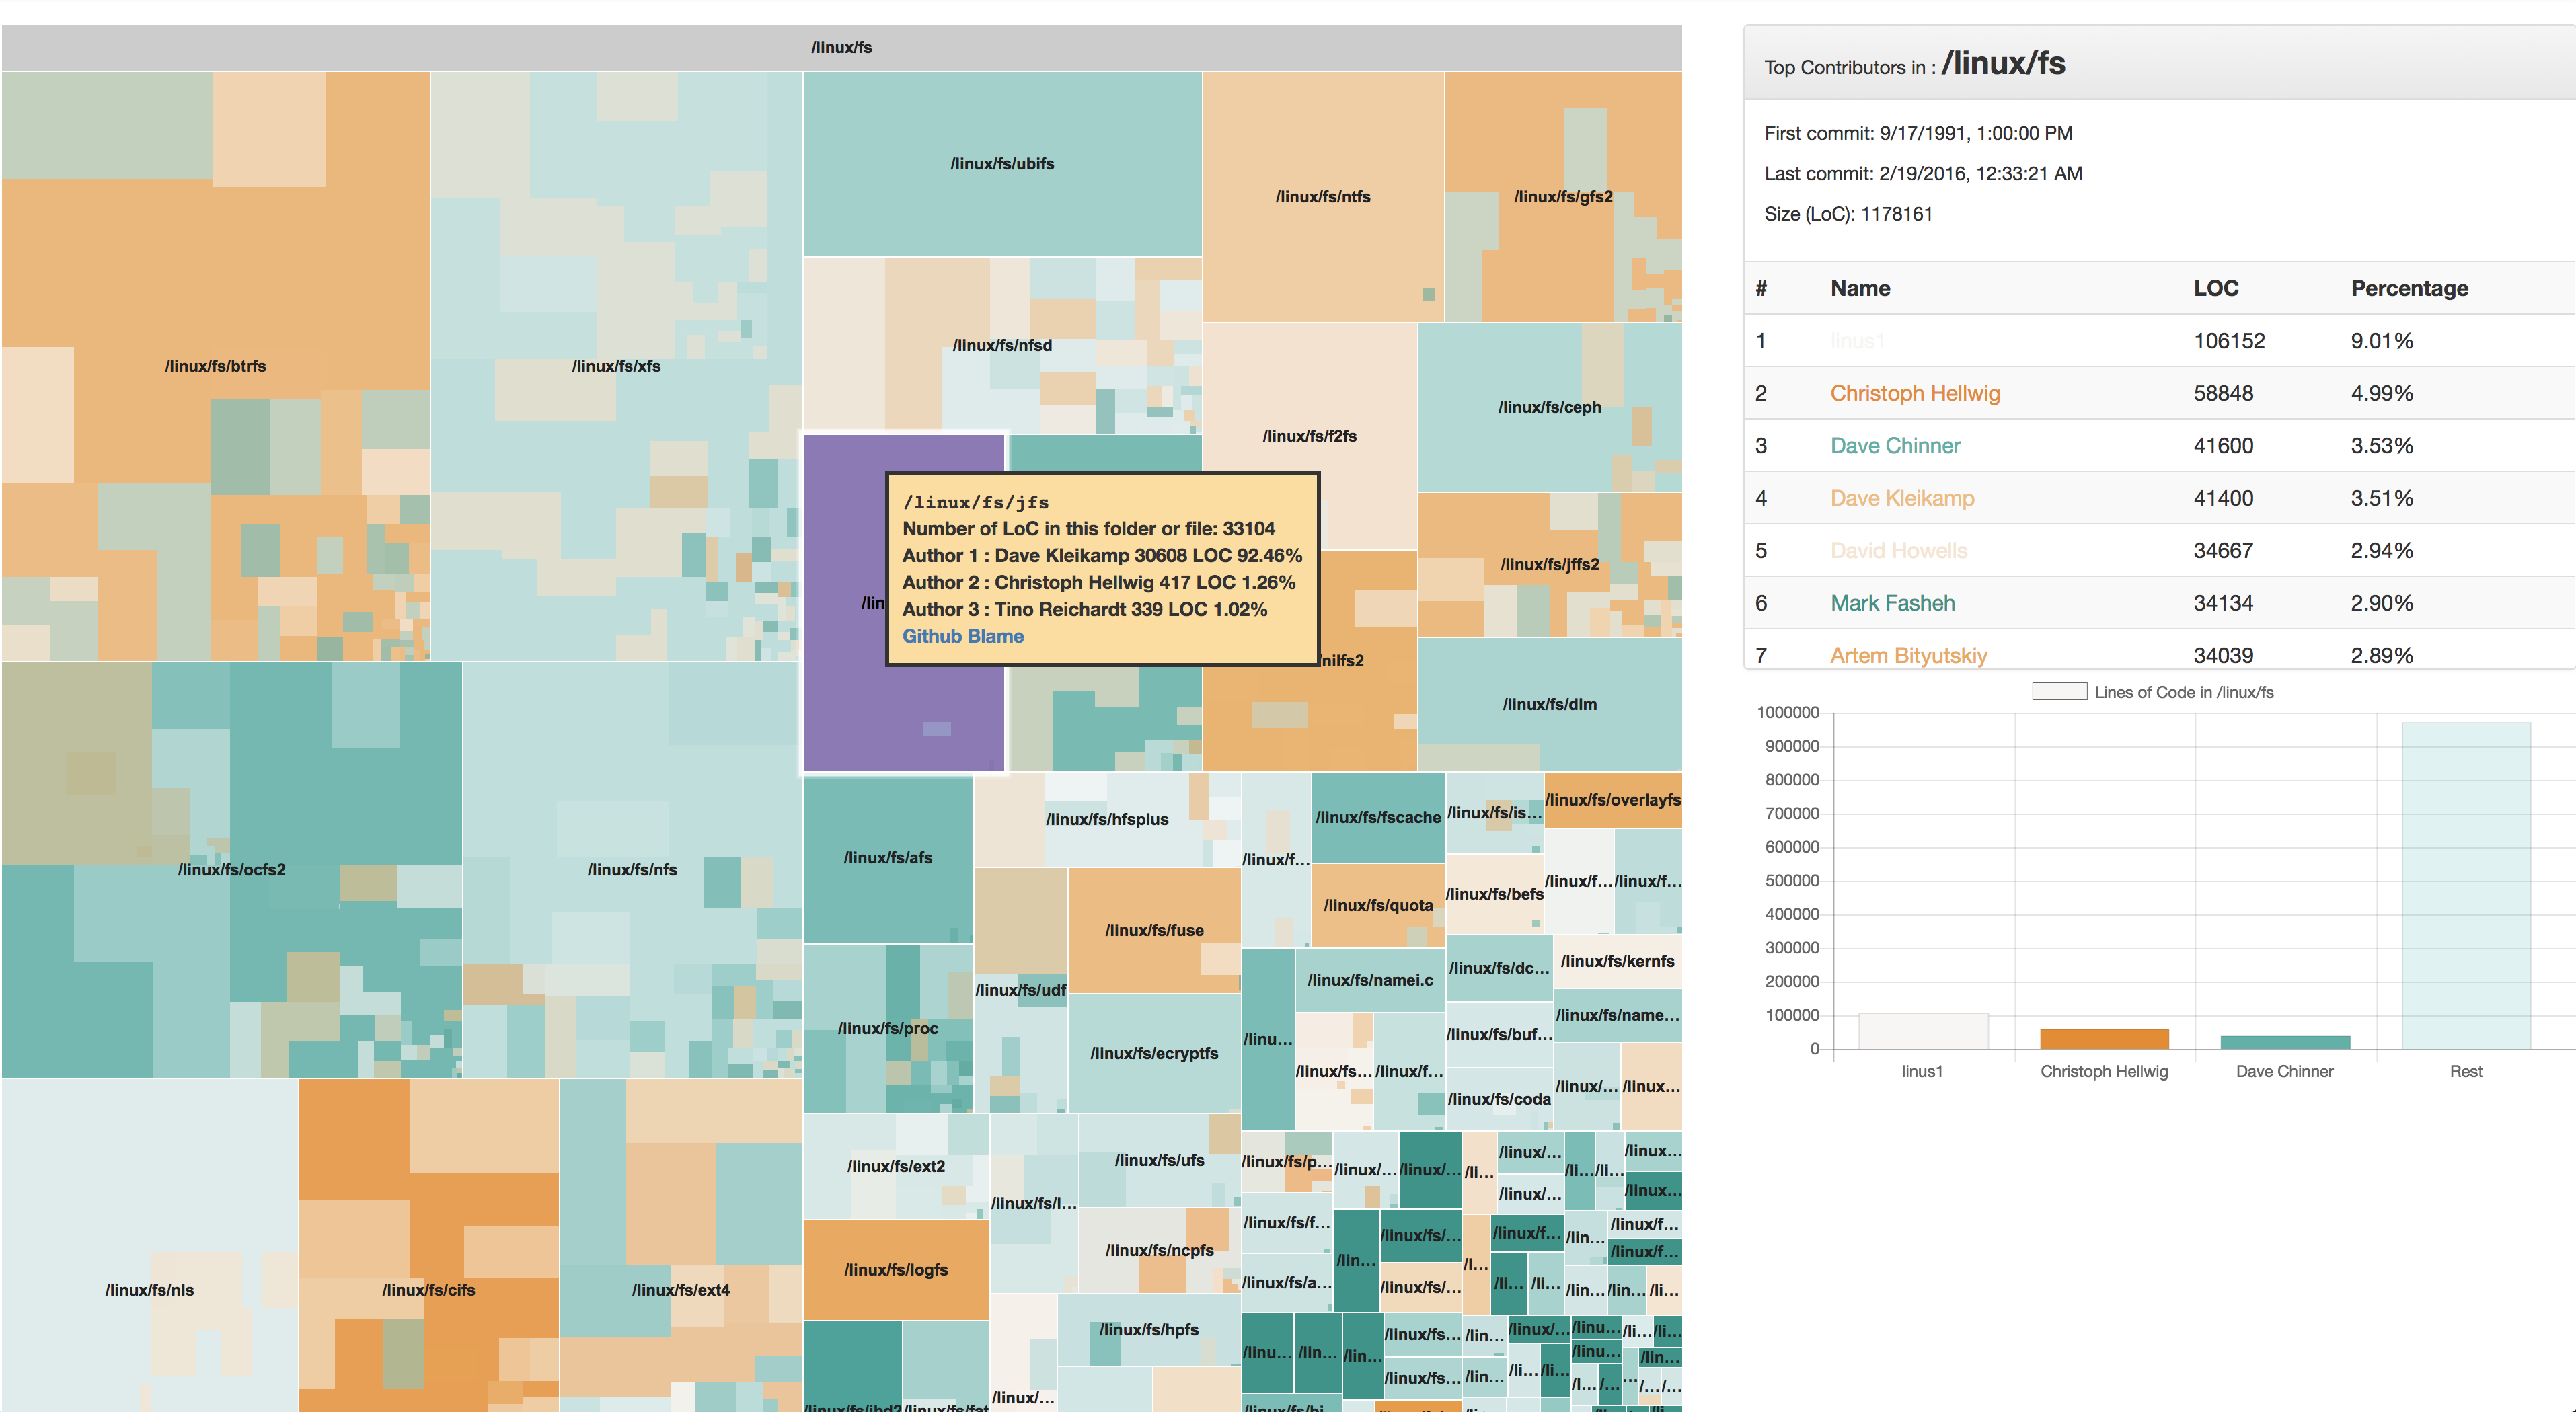
\includegraphics[width=5in]{srcmap1}
\caption{First version of srcmap}
\label{fig:srcmap1}
\end{figure}

\autoref{fig:srcmap1} shows the first version of Srcmap. The diferent boxes represent subdirectories of the Linux Kernel. The different colors present within each box give a preview of the content of the box. In this version of the tool, the color represents the developer having contributed the most lines of code in the contained files. Furthermore, the size of the boxes is proportional to the number of lines of code existing within the file or directory represented by the box. The panel on the right of the screen and the tooltip contain most of the data: exact number of lines of code, age of the first and last lines of code to be added, and the top 20 authors and their percentage of lines of code contributed.


\subsection{Srcmap 2.0}


After some research, we discovered a new treemap implementation\footnote{\url{https://carrotsearch.com/foamtree/}} capable of handling large dataset and deeply nested stuctures, which we used for the second version of the tool\footnote{\url{http://mcis.polymtl.ca/~courouble/dev/}}. This new version, shown in \autoref{fig:srcmap2}, introduced three important features: 
\begin{itemize}
	\item Coloring the files and directories according to three metrics:
	\begin{itemize}
		\item \ac{LOC}
		\item Median age
		\item Number of commits since 2016, or "Hot files"
	\end{itemize}
	\item File search
	\item A plot displaying the \textit{age} distribution of \ac{LOC} present in the file/directory.
\end{itemize}

\begin{figure}[htb]
\centering
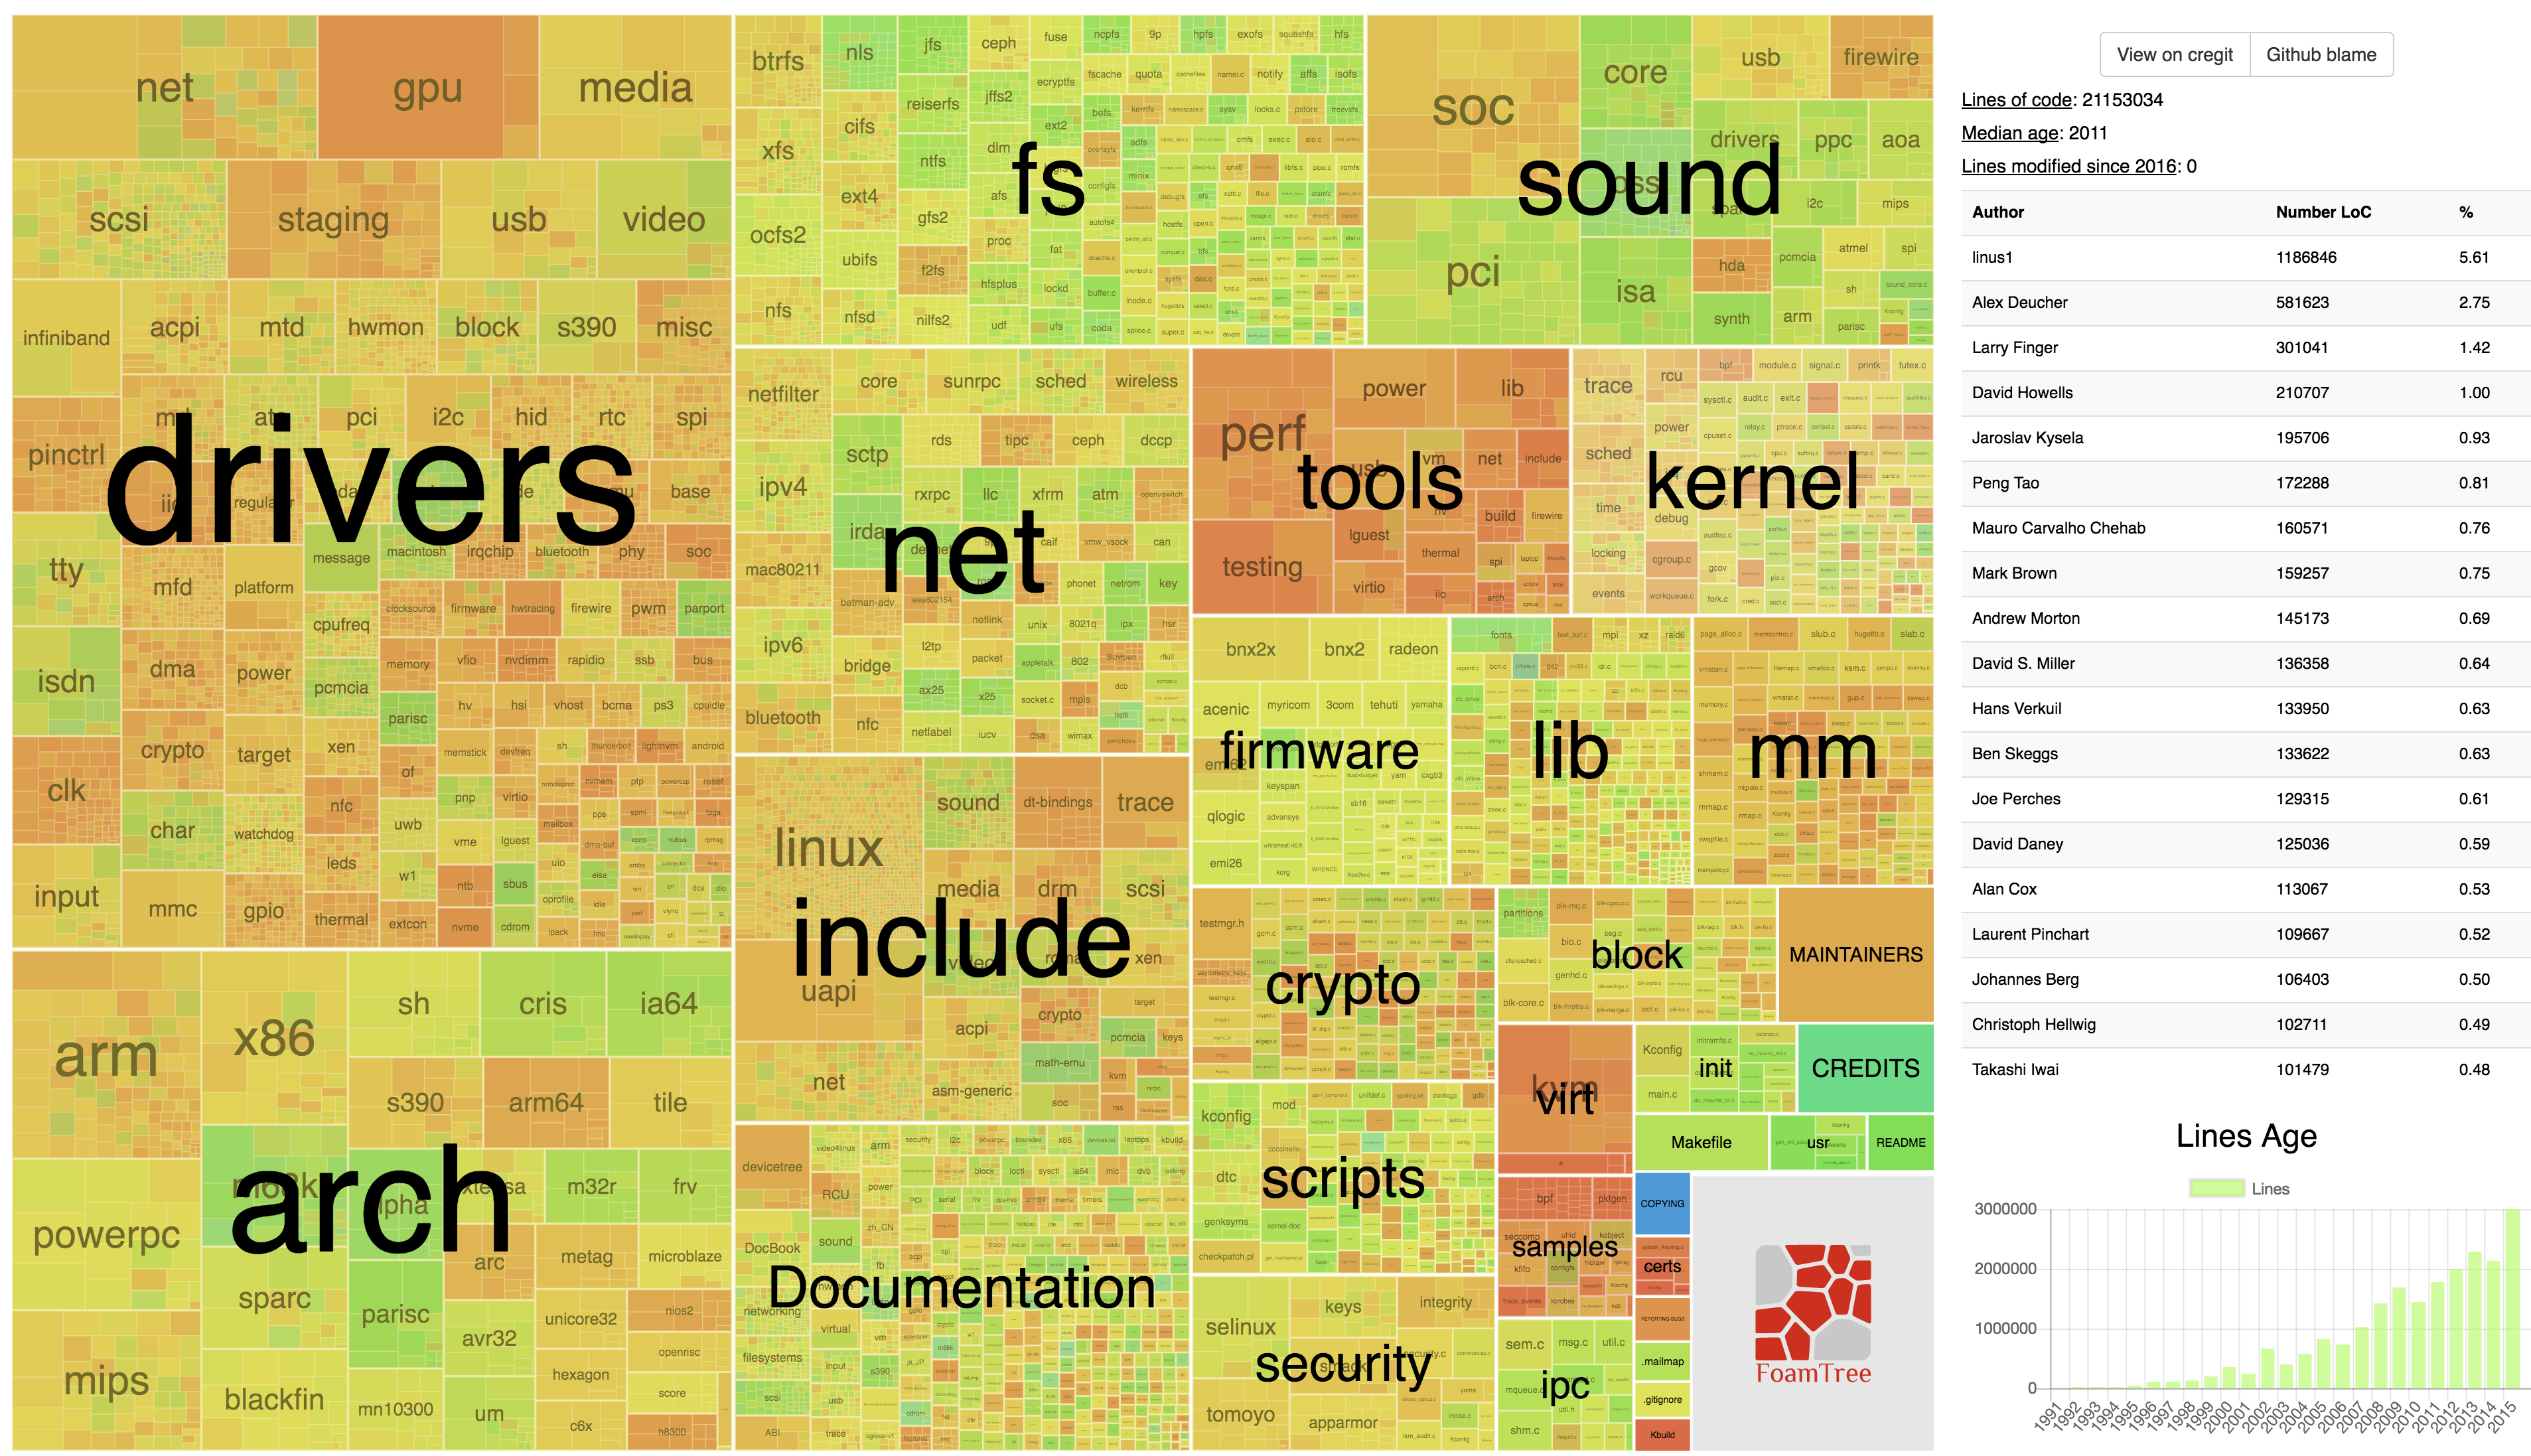
\includegraphics[width=5in]{srcmap2}
\caption{Second version of srcmap}
\label{fig:srcmap2}
\end{figure}

Although the foamtree library had a steeper learning curve than the Google Charts Treemap library, the versatility provided by the foamtree library allow us to provide a much more pleasant user experience and easier access to the data.


The very first Srcmap prototype consisted of a treemap displaying only the \texttt{net} subdirectory, which was small enough to provide a smooth user experience. However, Scalability issues started to arise when we attempted displaying the entire Linux Kernel source code. The data would take up to 30 seconds to load, and navigating between each node became very slow.


Furthermore, we discovered the limitations of Google Charts when we tried adding new features to the tool. The API provided did not allow the level of customization we desired. 


This is why we decided to create a new version of the tool with a different treemap library. The new library, Foamtree, provided a richer API and allowed for smooth browsing through deeply nested tree.





\subsection{Community Engagment}

After the creation of the first implementation of Srcmap, we attended LinuxCon 2016 to meet with a series of Linux developers and maintainers. The goal of these informal interviews was to recieve early feedback on the tool. In addition to that, I traveled to Santa Fe, New Mexico to present Srcmap at the Linux Plumbers Conference. After discussing srcmap and our research to a series of linux developers, we deducted the following. 

Firstly, experienced linux developers and maintainers are accustomed to their own development workflow. According to our interviews, experienced developers have acquired \textit{muscle memory} from developing in the same terminal over the years. Moreover, experienced maintainers were not interested in a web-based visualization tool, especially since the metrics displayed in Srcmap were easily accessible from the Linux git repository. In other words, the linux developers that I met show little interest in the tool. 

However, the interviewed developers showed interest in work that was previously done by \cite{jiang14}: linking Linux git commits to email patches and code reviews. Since our we wished to provide a tool that would increase developers' productivity, this became our next goal. Access to the original patches and code reviews would save a lot of time to developers trying to further understand an unknown code area. 



\subsection{Lessons learned}
\label{sec:lessons_srcmap}

We learned many important lesson during the creation of Srcmap.  From a community perspective, we now understand the importance of understanding the needs and the habits of the targetted community. 


From a research point of view, the creation of srcmap allowed us to understand an important concept in the creation of our expertise model. The different areas displayed in the treemap represent the footprint of the developer in the given area. In this case, the area represents a file or directory. As we updated srcmap to a newer release of the Linux Kernel, we noticed that the larger footprints were decreasing. Which lead us to discover the concept of decreasing footprint, an important aspect of our expertise model. 


In conclusion, although Srcmap was not as succeful as we originally hoped, we learned many important concepts that helped us in the rest of our research. 


\section{Email2git}
\label{sec:email2git}

The linux contribution process has been a reliable way to pipe code contributions (patches) from developers around the world, to the main Linux repository. With a working copy of the Linux Kernel on their computers, developer can modify the source code and, if desired, submit their changes for review, in hope to integrate the main tree. If accepted, the maintainer will \textit{commit} the changes to his local git repository, and submit the changes \textit{upstream} to another maintainer. 

Although this system has been very reliable, it has one major drawback: once committed, it is impossible to easily find the email conversation that eventually led to the creation of the patch. We addressed this drawback by implementing an algorithm capable of backtracking the origin of commits in the Linux Git repository introduced by~\citep{jiang14}. The algorithm and the issues related to scalability are described in chapter 4.

The data generated by the algorithm consists of a list of commit to patch matches. The matches are accessible online through two interfaces: as a commit ID search through the Email2git interface\footnote{\url{http://mcis.polymtl.ca/~courouble/email2git/}}, or though the Cregit interface\footnote{\url{https://cregit.linuxsources.org/}}.



\subsection{Integrating Email2git with Cregit}

Cregit is a project that aim at providing a finer grain approach to \textit{git blame}. The blame option in git returns the name of the developer who last changed a line of code in the source code. It provides a great way to quickly unmask the developers responsible for code in the Source Code. However, it has a serious limitation: git blame assigns a line to a developer even after a small modification to that line. For instance, if developer $A$ writes \texttt{print "Hello world"}, this line will then become associated with developer $A$. However, if developer $B$ modifies the line to read \texttt{print "Hello world!"}, git blame will associate the line with devloper $B$ even though developer $B$ only added a character. 

Cregit addresses this limitation by tokenizing the source code in a git repository to enables git blame at a token level, instead of a line level. This provides a better understanding of the true authors of the source code. A tokensize version of the Linux kernel source code is available online through the cregit interface\footnote{\url{https://cregit.linuxsources.org/}}.

\begin{figure}[htb]
\centering
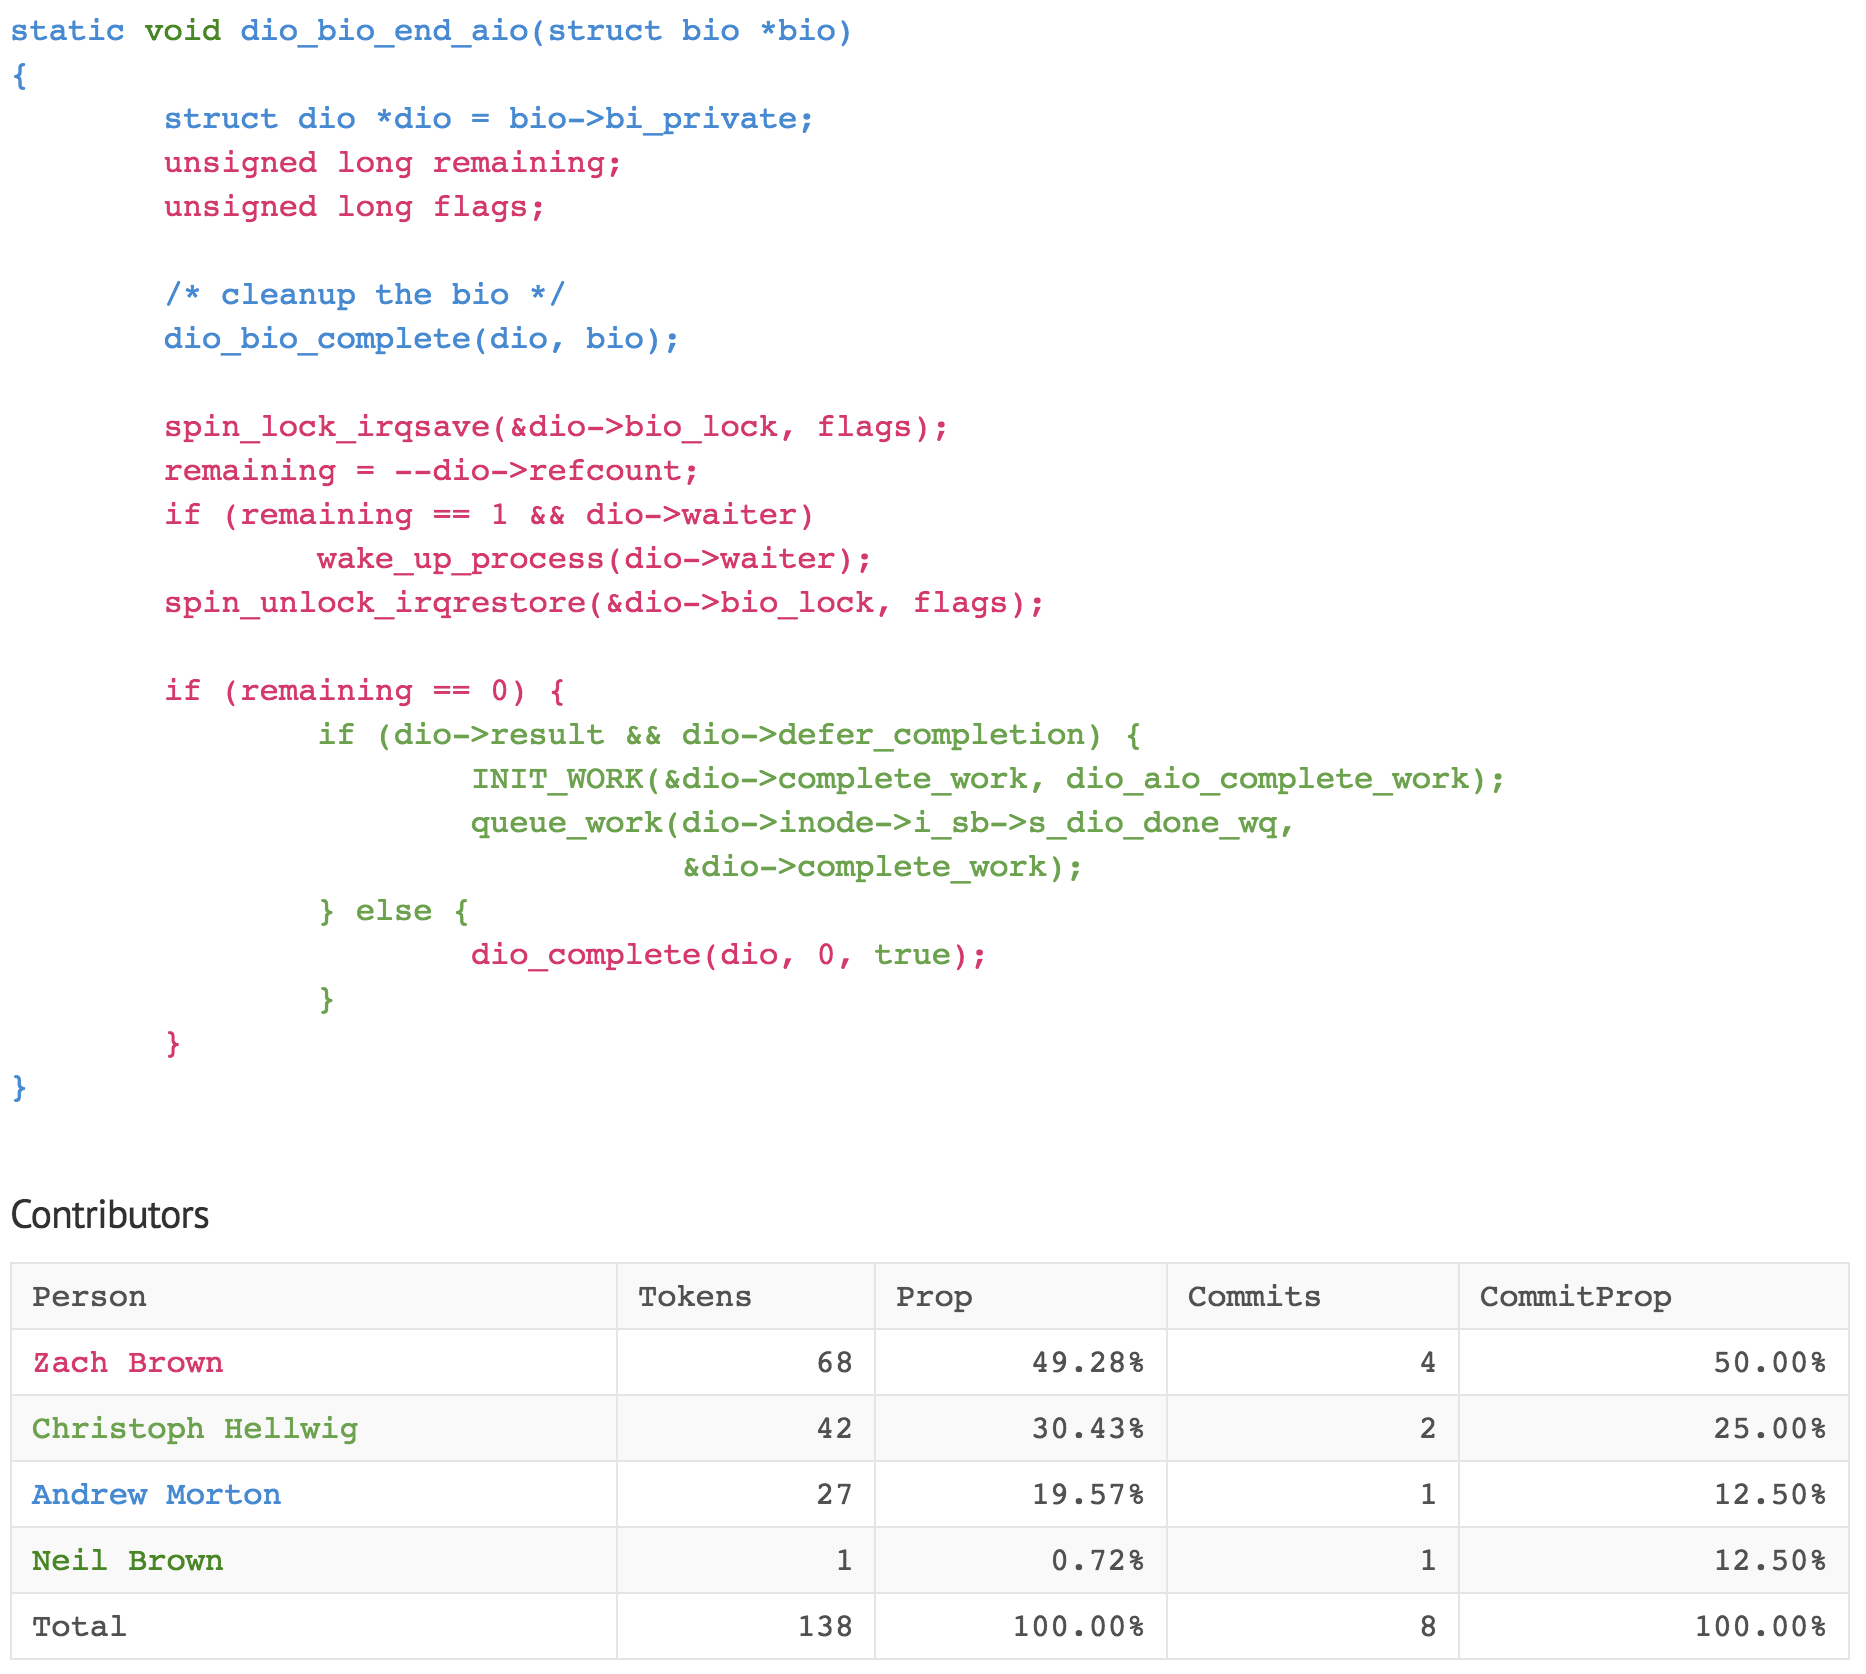
\includegraphics[width=3.5in]{cregit_code}
\caption{Tokenized source code as it appears on Cregit.}
\label{fig:cregit_code}
\end{figure}

\autoref{fig:cregit_code} shows tokenized linux code as it appears on the Cregit interface. In an effort to ease the access to email2git data, we decided to provide access to the matches through cregit. To this end, I modified the user interface to display a window containing all the available patches after clicking on a token, as shown in \autoref{fig:cregit_matches}. 

\begin{figure}[htb]
\centering
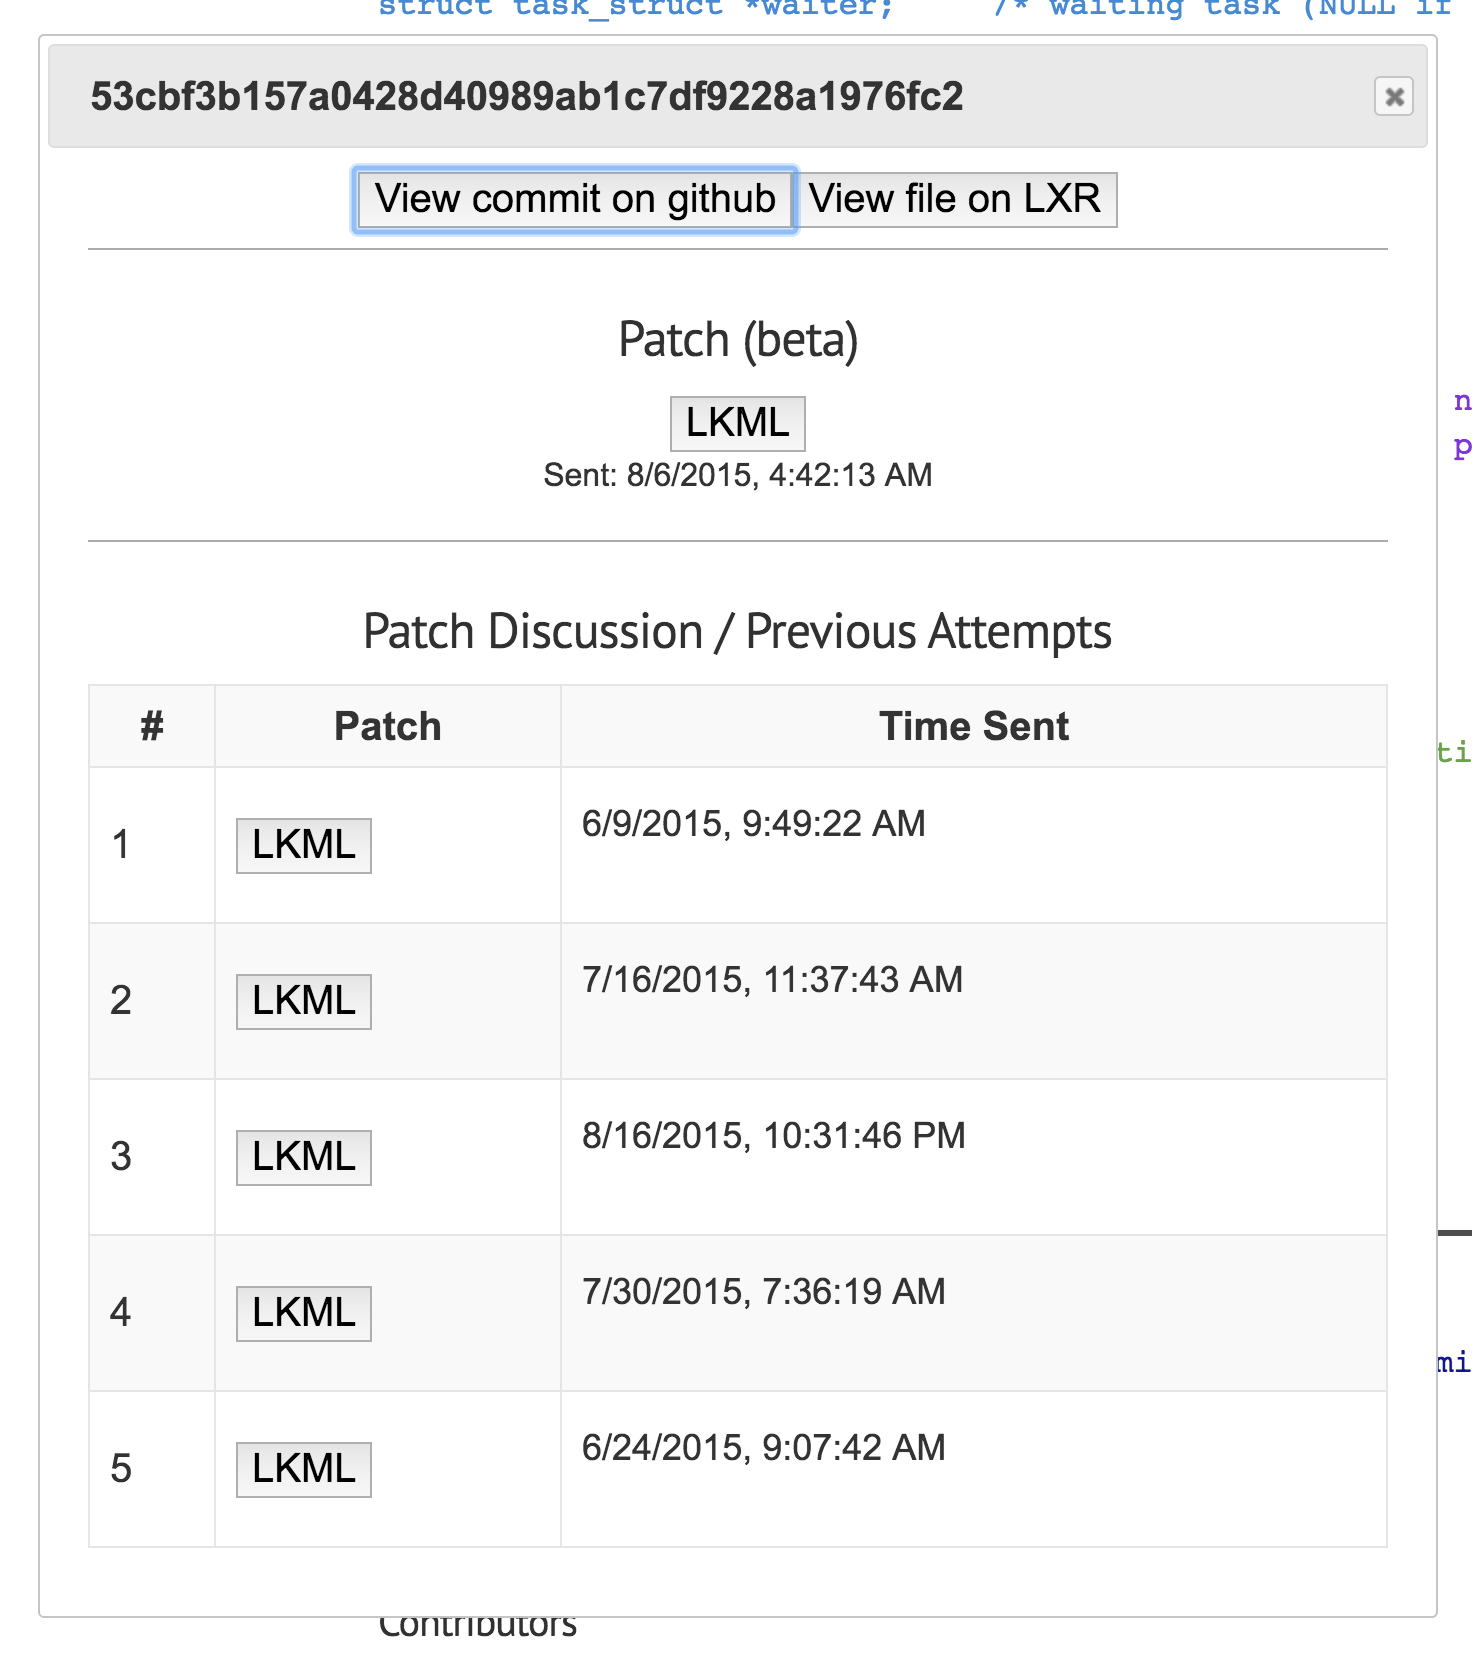
\includegraphics[width=3.5in]{cregit_matches}
\caption{Window containing the patches that introduced the commit associated with the clicked token}
\label{fig:cregit_matches}
\end{figure}







\subsection{Lessons Learned}


We leveraged the lessons learned from Srcmap while creating Email2git. The purpose of Email2git was to answer a complain coming from multiple developers and maintainers: the difficulty of finding an email discussion about patches that were eventually integratted in the Linux Kernel. Understanding the Linux community allowed us to better introduce our tool when we released it, as explained in Chapter 4. Moreover, the data acquired in the implementation of Email2git served as one of the metrics used by our expertise model as explained in chapter 5.





